\chapter{Лабораторная работа 3}
\section*{Практическое задание}

Целью лабораторной работы №3 является отработка навыков использования программы Microsoft Project для оптимизации временных и финансовых показателей проекта.

\textbf{Содержание проекта:} команда разработчиков из 16 человек занимается созданием карты города на основе собственного модуля отображения. Проект должен быть завершен в течение 6 месяцев. Бюджет проекта: 50 000 рублей.

Команда проекта состоит из 5 программистов (из них 1 ведущий), Web-дизайнера, системного аналитика, 5 наборщиков данных, 2 дизайнеров, технического писателя и медиа-корреспондента.

\subsection*{Задание 1}

На начало работы в проекте присутствуют перегрузки ресурсов: 

\begin{figure}[h!]
	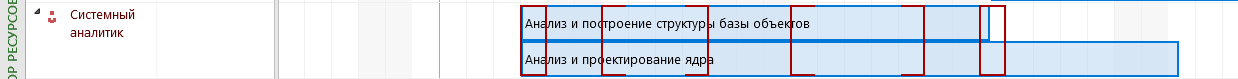
\includegraphics[scale=0.4, center]{lab02_task2_3_1}
\end{figure}

\begin{figure}[h!]
	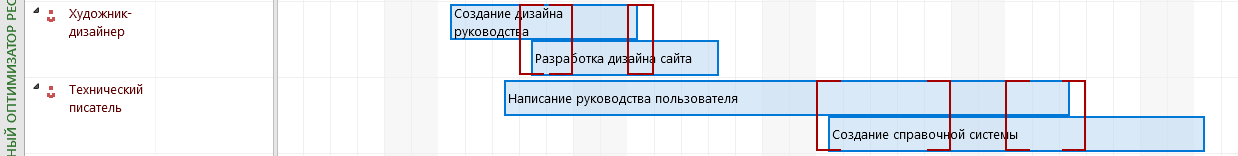
\includegraphics[scale=0.4, center]{lab02_task2_3_2}
\end{figure}


Нагрузка была ликвидирована при помощи автоматического выравнивания (по часам):

\begin{figure}[h!]
	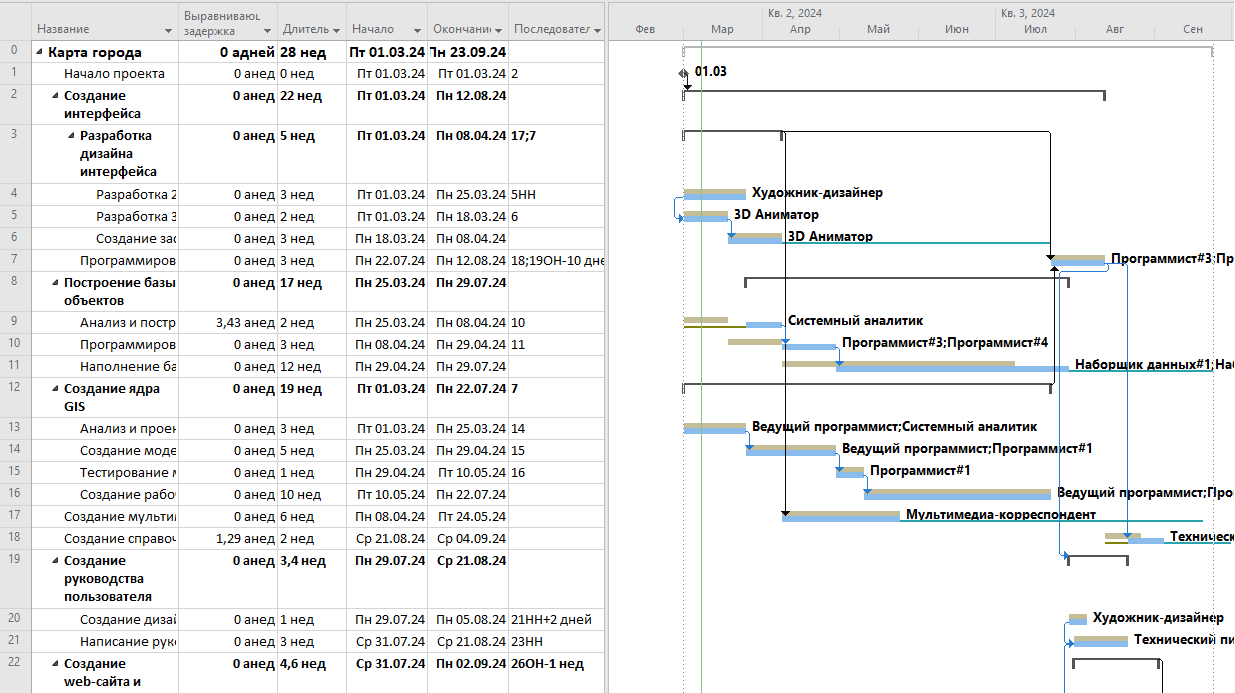
\includegraphics[scale=0.4, center]{lab03_task1_1}
\end{figure}


Дата завершения проекта изменилась с 19 сентября на 23 сентября, это произошло из-за того, что длительность разработки дизайна сайта увеличилась на 4 дня (художник-дизайнер в это время занят созданием дизайна руководства пользователя, и у Web-дизайнера и 3D аниматора на выполнение работы уходит больше времени).

Стоимость проекта уменьшилась с 48 270 рублей до 48 124 рубля из-за того, что на 73 часа уменьшилось время работы сервера (из-за появления выравнивающей задержки для задачи анализа и построения структуры базы данных).

\clearpage
\subsection*{Задание 2}

Было добавлено совещание по средам длительностью 1 час:
\begin{figure}[h!]
	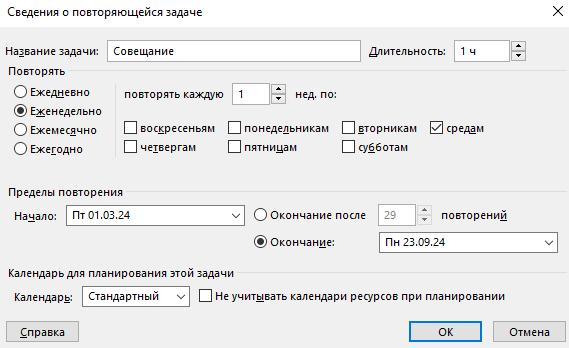
\includegraphics[scale=0.6, center]{lab03_task2_1}
\end{figure}

Были назначены ресурсы для всех совещаний:
\begin{figure}[h!]
	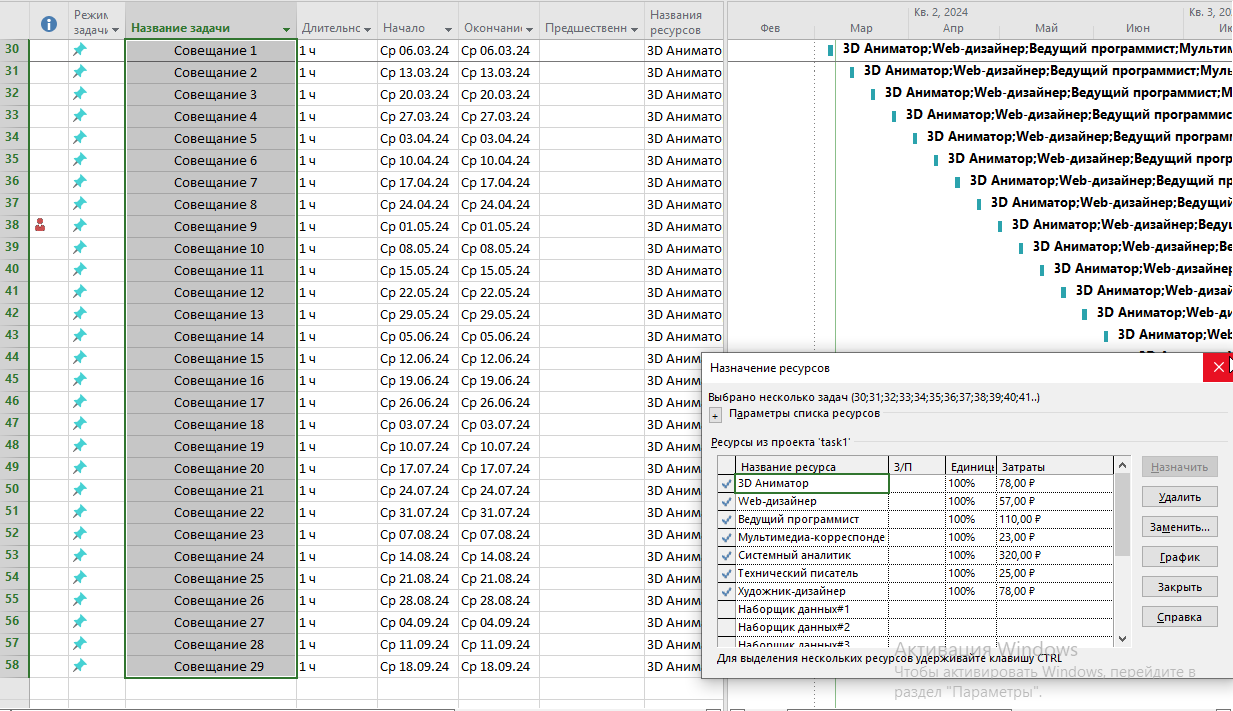
\includegraphics[scale=0.4, center]{lab03_task2_2}
\end{figure}

Возникла перегрузка ресурсов из-за того, что одновременно выполнялись совещания и другие задачи. Решить данную проблему можно выравниванием с включённой опцией ''При выравнивании допускается прерывание оставшихся трудозотрат'', в таком случае задачи будут прерываться на совещание (из-за того, что приоритет совещания выше).

После выравнивания дата окончания проекта сместилась на 25 сентября, а стоимость проекта составила 68 165 рублей.

Вернуть стоимость проекта в пределы 50 000 можно, назначив совещаниям другую таблицу норм.затрат (например, В).

%\begin{figure}[h!]
%	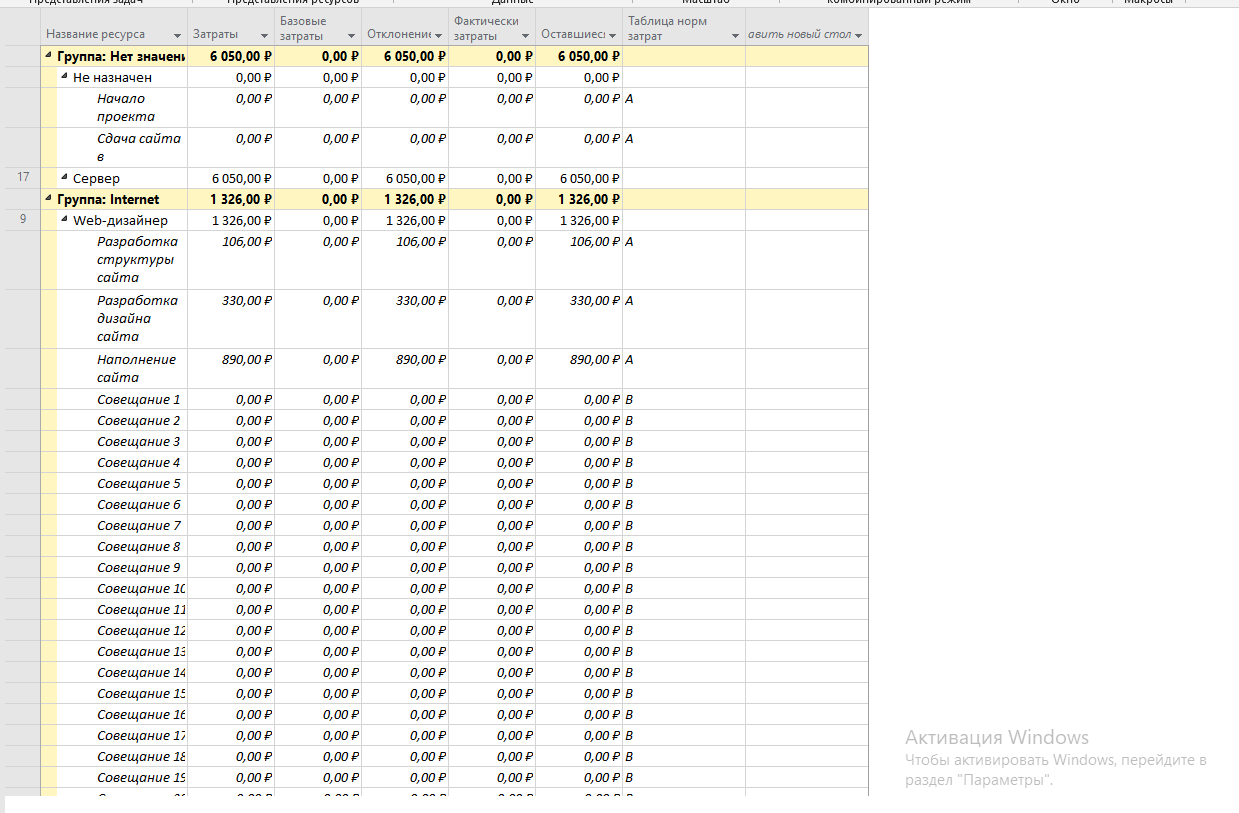
\includegraphics[scale=0.4, center]{lab03_task2_3}
%\end{figure}

\clearpage
\subsection*{Задание 3}

При помощи фильтра отобразим критические задачи:

\begin{figure}[h!]
	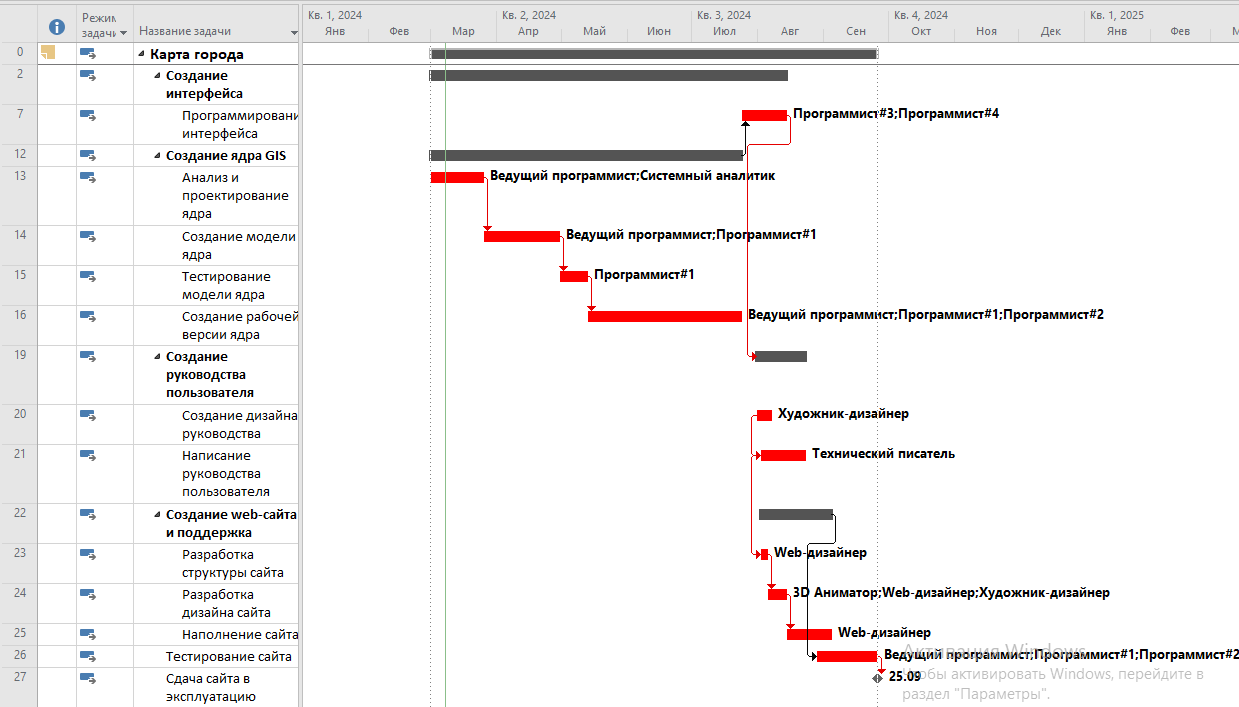
\includegraphics[scale=0.4, center]{lab03_task3_1}
\end{figure}
\clearpage

Значительная задержка происходит из-за того, что при создании рабочей версии ядра используются не все программисты. Если это исправить, длительность проекта получится уменьшить на месяц (дата окончания проекта - 17 августа). Это также поможет снять нагрузку с ведущего программиста и уменьшить стоимость проекта до 49 494 рублей.
\begin{figure}[h!]
	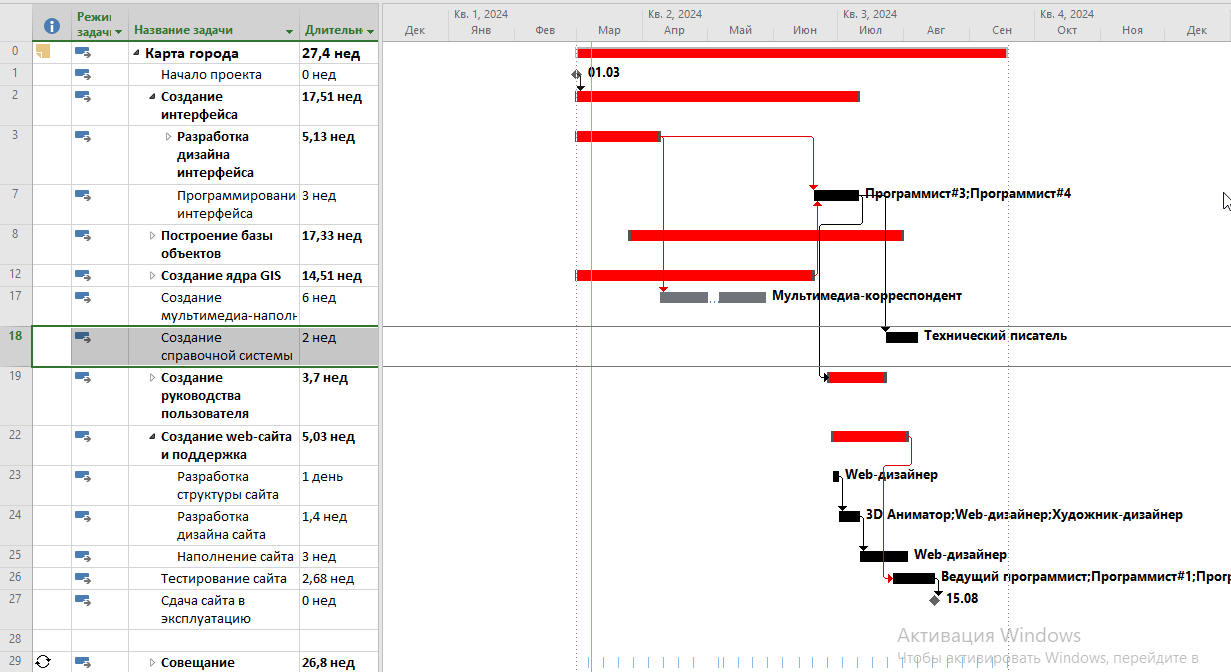
\includegraphics[scale=0.4, center]{lab03_task3_2}
\end{figure}

Сравним диаграммы для расчёта процентного соотношения затрат и трудозатрат в лабораторных 2 и 3.
\clearpage

\begin{figure}[h!]
	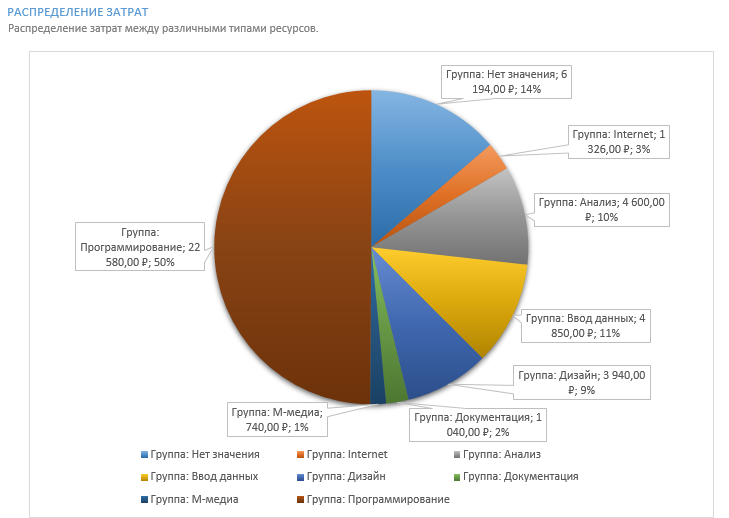
\includegraphics[scale=0.6, center]{lab02_task3_2}
\end{figure}

\begin{figure}[h!]
	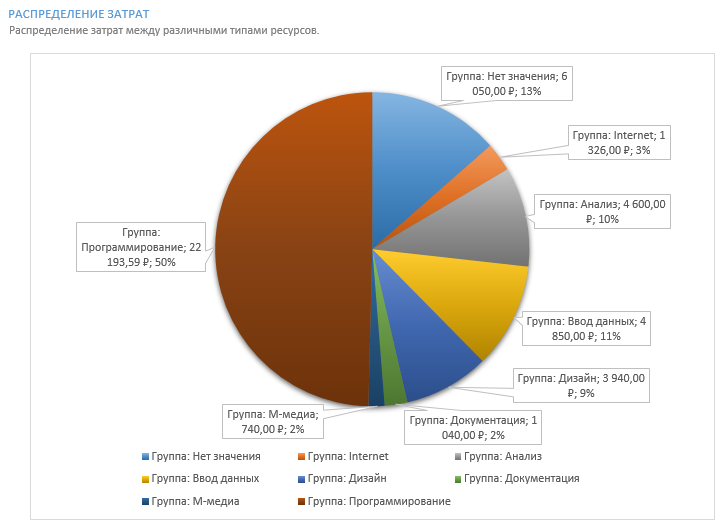
\includegraphics[scale=0.6, center]{lab03_task3_3}
\end{figure}

\clearpage

\begin{figure}[h!]
	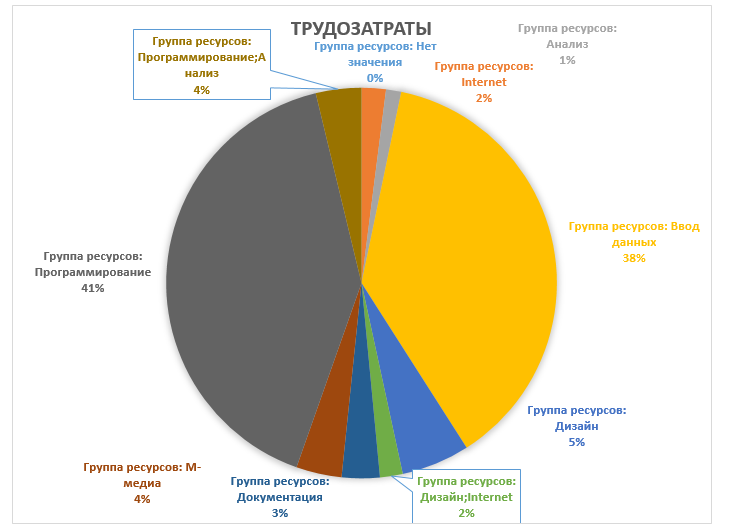
\includegraphics[scale=0.6, center]{lab02_task3_3}
\end{figure}


\begin{figure}[h!]
	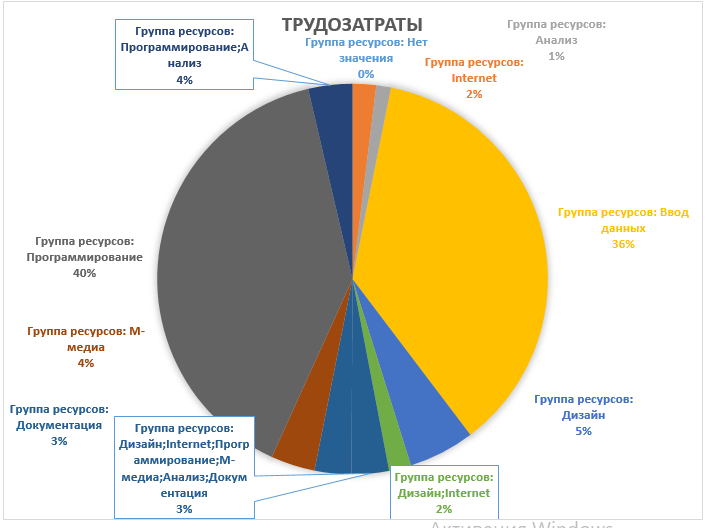
\includegraphics[scale=0.6, center]{lab03_task3_4}
\end{figure}

Был сохранён базовый план проекта:

\begin{figure}[h!]
	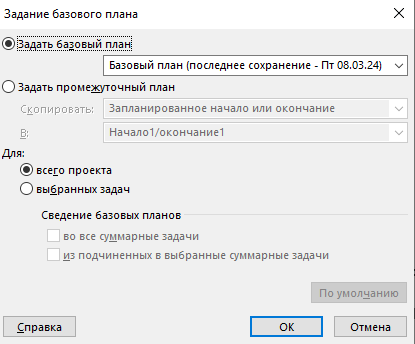
\includegraphics[scale=0.8, center]{lab03_task3_5}
\end{figure}

\section*{Заключение}

В ходе выполнения данной лабораторной работы были отработаны навыков использования программы Microsoft Project для оптимизации временных и финансовых показателей проекта.

В результаты затраты по проекту равны 49 494 рублей (укладывается в бюджет).
Посредством использования программистов в задаче по разработке ядра удалось снять нагрузку с вещущего программиста и уменьшить длительность проекта на месяц - теперь дата завершения проекта 17 августа (укладывается в срок).